%
% LaTeX Report Assignment 4
% Applied Programming Lab EE2703
% Ayush Jamdar EE20B018 
%


\documentclass[11pt, a4paper]{article}
\usepackage{graphicx}
\usepackage{amsmath}
\usepackage{listings}
\usepackage[]{courier}


\title{Assignment 4: Fourier Approximations} % Title

\author{Ayush Jamdar EE20B018} % Author name

\date{\today} % Date for the report
\begin{document}		
		
\maketitle % Insert the title, author and date
\section{Aim}
%Create new section;it is autonumbered
The goal of this assignment is to fit the functions, $exp(x)$ and $cos(cos(x))$ over the interval $[0, 2\pi)$ using the trigonometric fourier series
$$a_{0}+\sum_{n=1}^{\infty}{a_{n}cos(nx)+b_{n}sin(nx})$$
where the coefficients are given by
\[a_{n}=\frac{1}{2\pi}\int_{0}^{2\pi} f(x)\cos(nx) \,dx \]
\[b_{n}=\frac{1}{2\pi}\int_{0}^{2\pi} f(x)\sin(nx) \,dx \]


\section{The Assignment}

 \subsection{Question 1: Getting the functions}
 I start by defining Python functions for each of the two functions. These functions return \texttt{numpy} arrays. Note that \texttt{numpy} has been imported under the alias \texttt{np}.
 \begin{verbatim}
 def exponential(x):
    return np.exp(x)

 def coscos(x):
    return np.cos(np.cos(x))
 \end{verbatim}
 Now, I plot each of them over the range $[-2\pi, 4\pi)$ in two ways - the actual function and the periodic extension with a $2\pi$ period. Note that $e^x$ has been plotted on a semilog scale. The following Python code does this (and similarly for $\cos(\cos(x))$):
 	\begin{verbatim}
 	x = np.linspace(-2 * np.pi, 4 * np.pi, 300)
	y1 = exponential(x)
	y1_periodic = y1[100: 200]
	y1_periodic = np.append(y1_periodic, y1_periodic)
	y1_periodic = np.append(y1_periodic, y1[100: 200])  
	# because I am plotting over three periods
	
	semilogy(x, y1, 'red', label='Main function')
	semilogy(x, y1_periodic, label='Periodic over 0 to 2\u03C0')
	grid()
	xlabel("x")
	ylabel("e^x")
	legend()
	title("Q1: Exponential(x)")
	show()
 	\end{verbatim}
 
   \begin{figure}[!tbh]
   	\centering
   	  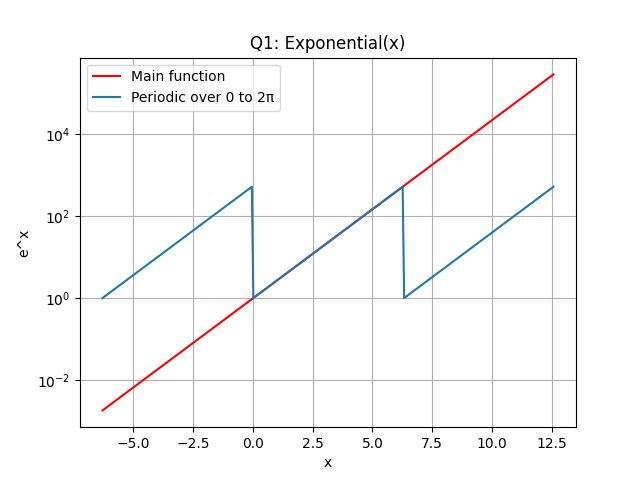
\includegraphics[scale=0.5]{q1-f1.png} 
     \caption{Q1: The Exponential Function}
   	\label{fig:Q1-f1}
   \end{figure}

   \begin{figure}[!tbh]
   	\centering
   	  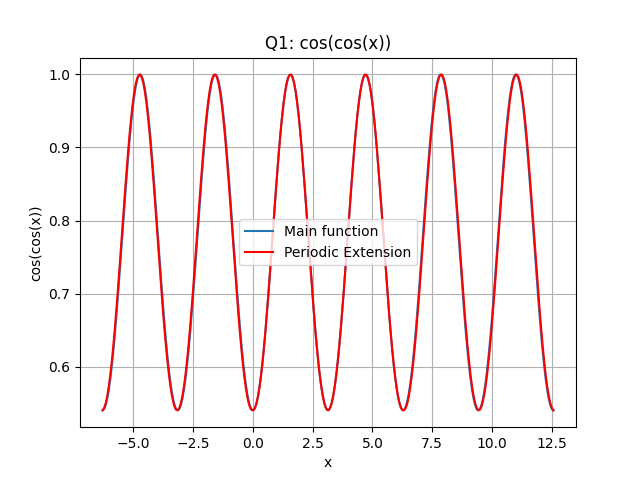
\includegraphics[scale=0.5]{q1-f2.png} 
    \caption{Q1: The $cos(cos(x))$ Function}
   	\label{fig:Q1-f1}
   \end{figure}
	\newpage
    As one may observe, the periodic extension of $\cos(\cos(x))$ matches the actual function because it is inherently periodic.
    
    
  \subsection{Question 2: Building the Fourier Series}
  The goal is to obtain 51 coefficients for each of the two functions. The Fourier coefficients, in order, $a_{0}, a_{1}, b_{1}, \ldots{},a_{25}, b_{25}$. I have created two new functions to be integrated, namely \texttt{f(x, k)} and \texttt{g(x, k)} . This is implemented for the exponential function in the below code block. Note that $k$ is the second argument of the function. The integrator function \texttt{integrate.quad} from the scipy module integrates its first argument (integrand) from limits $0$ to $2\pi$; the fourth argument passes $k$ to the function \texttt{f(x, k} (or \texttt{g(x, k)}).
     
  \begin{verbatim}
f0 = lambda a: np.exp(a)
a0_exp = (scipy.integrate.quad(f0, 0, 2 * np.pi)[0])/(2 * np.pi)

   # 'a' coefficients for this series
a_n_exp = []
for i in range(1, 26):
    f = lambda x, k: np.exp(x) * np.cos(x * k)
    a_n_exp.append((scipy.integrate.quad(f, 0, 2 * np.pi,
     args=(i))[0]) / np.pi)

b_n_exp = []
for i in range(1, 26):
    g = lambda x, k: np.exp(x) * np.sin(x * k)
    b_n_exp.append((scipy.integrate.quad(g, 0, 2 * np.pi,
     args=(i))[0]) / np.pi)

  \end{verbatim}  
  And for the $cos(cos(x))$ function,
  \begin{verbatim}
  p0 = lambda x: np.cos(np.cos(x))
a0_cos = (scipy.integrate.quad(p0, 0, 2 * np.pi)[0]) / (2 * np.pi)

a_n_cos = []
for i in range(1, 26):
    p = lambda x, k: np.cos(np.cos(x)) * np.cos(x * k)
    a_n_cos.append((scipy.integrate.quad(p, 0, 2 * np.pi,
     args=(i))[0]) / np.pi)

b_n_cos = []
for i in range(1, 26):
    q = lambda x, k: np.cos(np.cos(x)) * np.sin(x * k)
    b_n_cos.append((scipy.integrate.quad(q, 0, 2 * np.pi,
     args=(i))[0]) / np.pi)

  \end{verbatim}  
  The coefficients $a_{n}$ and $b_{n}$ are plotted.
  \begin{figure}[!tbh]
   	\centering
  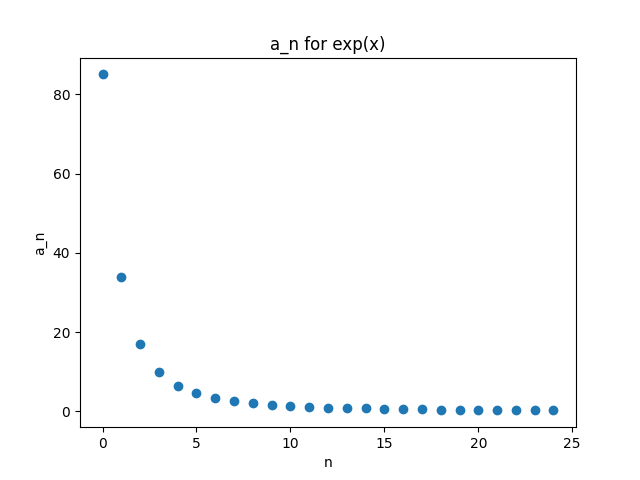
\includegraphics[scale=0.5]{an-exp.png} 
    \caption{Q3: $a_{n}$ for $exp(x)$}
   	\label{fig:an for exp(x)}
   \end{figure}
   
   \begin{figure}[!tbh]
   	\centering
  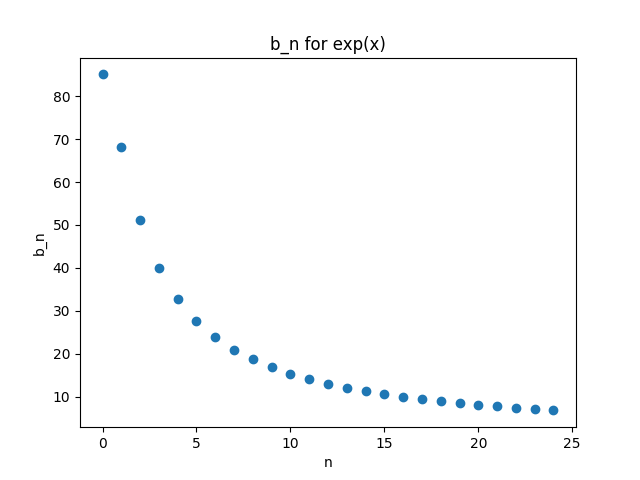
\includegraphics[scale=0.5]{bn-exp.png} 
    \caption{Q3: $b_{n}$ for $exp(x)$}
   	\label{fig:bn for exp()}
   \end{figure}
   
   \begin{figure}[!tbh]
   	\centering
  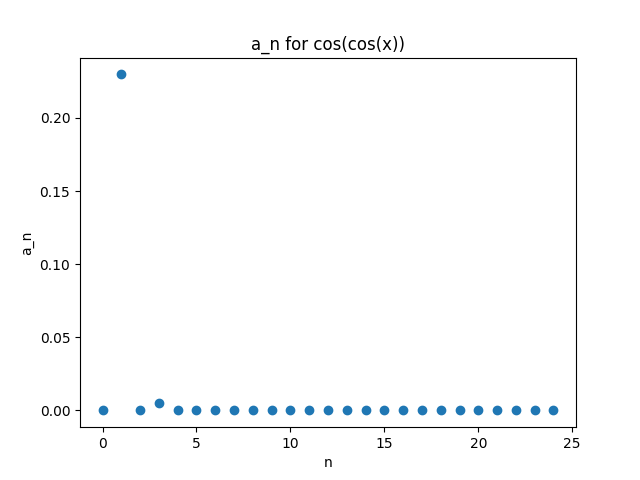
\includegraphics[scale=0.5]{an-cos.png} 
    \caption{Q3: $a_{n}$ for $cos(cos(x))$}
   	\label{fig:an for coscos()}
   \end{figure}
	
	\begin{figure}[!tbh]
   	\centering
  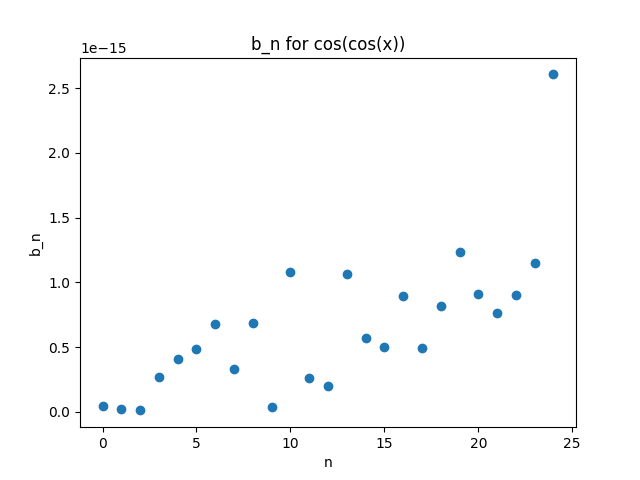
\includegraphics[scale=0.5]{bn-cos.png} 
    \caption{Q3: $b_{n}$ for $cos(cos(x))$}
   	\label{fig:bn for coscos()}
   \end{figure}
   
  \newpage
  \subsection{Question 3: Plotting the coefficients}
  For each of the two functions, I have plotted the Fourier coefficients' magnitude - once on a \texttt{semilog} scale and once on a \texttt{loglog} scale. Note that the order of coefficients on the x-axis (For the figures with 'Q3' in the caption) is $a_{0}, a_{1}, b_{1}, \ldots{},a_{25}, b_{25}$.\\
  First, the Fourier coefficients of $exp(x)$.
  
  \begin{figure}[!tbh]
   	\centering
  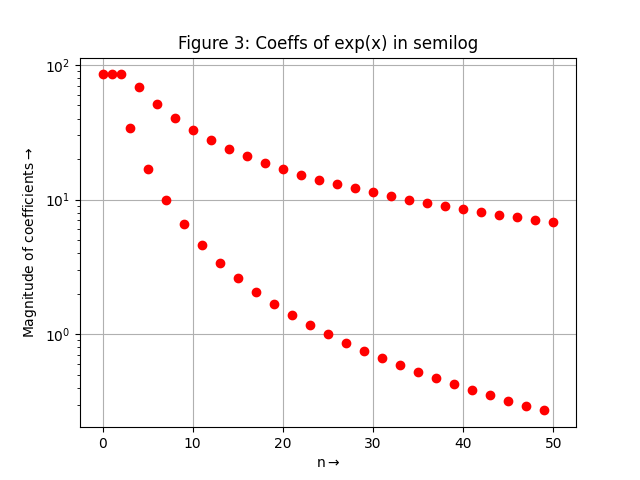
\includegraphics[scale=0.5]{q3-f1-semilog.png} 
    \caption{Q3: Coefficients of $exp(x)$}
   	\label{fig:Q3-f1-semilog}
   \end{figure}

\newpage   
   
  \begin{figure}[!tbh]
   	\centering 
  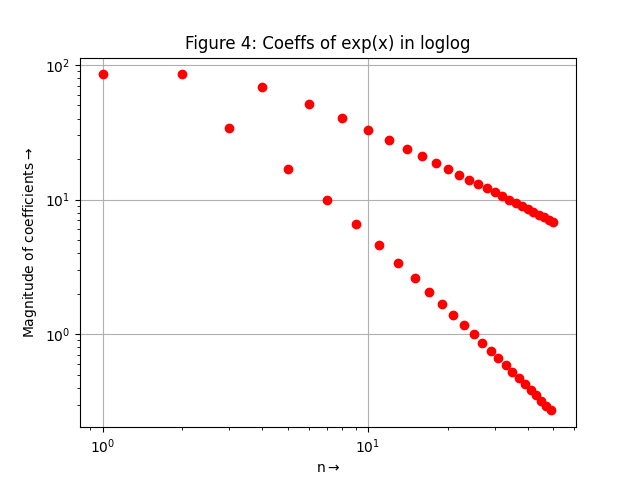
\includegraphics[scale=0.5]{q3-f1-loglog.png} 
    \caption{Q3: Coefficients of $exp(x)$}
   	\label{fig:Q3-f1-loglog}
   \end{figure}

 Next, the Fourier coefficients of $cos(cos(x))$.
   \begin{figure}[!tbh]
   	\centering
  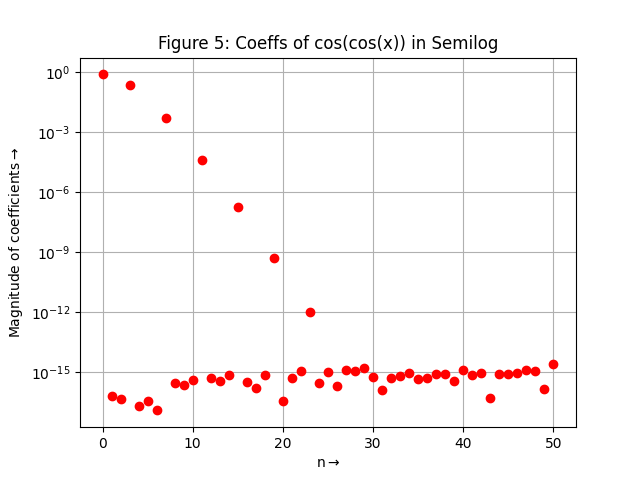
\includegraphics[scale=0.5]{q3-f2-semilog.png} 
    \caption{Q3: Coefficients of $cos(cos(x))$}
   	\label{fig:Q3-f2-semilog}
   \end{figure}
   
   
  \begin{figure}[!tbh]
   	\centering 
  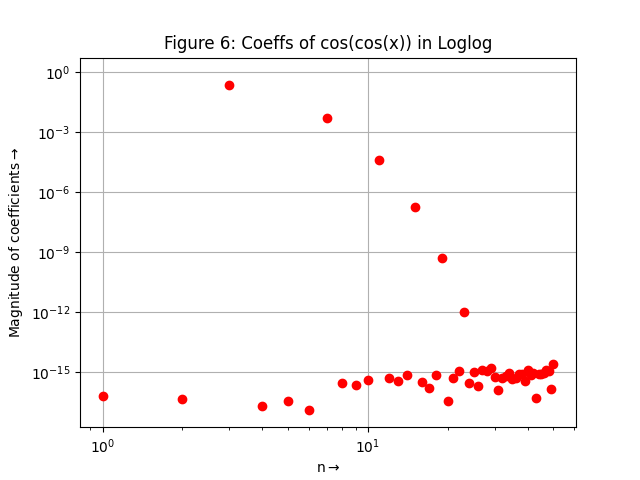
\includegraphics[scale=0.5]{q3-f2-loglog.png} 
    \caption{Q3: Coefficients of $cos(cos(x))$}
   	\label{fig:Q3-f2-loglog}
   \end{figure}

   The order of magnitude tells a lot about the nature of the series, where the harmonic contribution is significant and where it is not.
   \begin{enumerate}
   \item $b_{n}$ coefficients are observed in Figure 6. The y-axis numbers are on a $10^{-15}$ scale - nearly zero. The reason is, the function period is $2\pi$ and I am integrating it over 0 to $2\pi$. If I change the integration variable to $t+\pi$, limits will change from $-\pi$ to $\pi$, the integrand will remain the same (may get a +/- sign). The function $\cos(\cos(x))\sin(nx)$ is now an odd function. Hence, the integral should vanish. I obtain very tiny values because I used a finite number of $x$ for the integration function \texttt{quad}.  
   \item The reason why the coefficients of $e^x$ do not decay as quickly as that of $cos(cos(x))$ is - the latter is inherently periodic. In the Fourier domain, it will have a finite number of frequencies making up the signal. On the contrary, $e^x$ is not, hence, it is discontinuous at $2m\pi$.
   \item Fourier coefficients for $e^x$ are 
   $$a_{n}=\frac{e^{2\pi}-1}{(n^2+1)\pi}$$ 
   $$b_{n}=\frac{n-n{e^{2\pi}}}{(n^2+1)\pi}$$ 
   At large values of n, $log(a_{n})$ and $\log(b_{n}$ can be approximated as $-2\log(n)$ and $-\log(n)$ respectively. Hence the \texttt{loglog} plot is linear. Whereas the \texttt{semilog} plot in (caption) Figure 9 looks linear because the coefficients vary approximately as exponential $n$. 
    
   \end{enumerate}
   
   \subsection{Question 4 and 5: The Least Squares Approach}
   I have defined a vector \texttt{X} going from 0 to $2\pi$ in 400 steps. Lets deal with $e^x$ first. The function $e^x$ at these \texttt{X} values is given by another vector \texttt{b\_matrix\_for\_exp}. Now I build the matrix \texttt{A\_mat\_for\_exp}; the code is as follows:
   \begin{verbatim}
   X = np.linspace(0, 2*np.pi, 400)
   b_matrix_for_exp = exponential(X)
   X = np.linspace(0,2*np.pi,401)
   X = X[:-1] # drop last term to have a proper periodic 
      integral
   b_matrix_for_exp = exponential(X)  
   # f has been written to take a vector
   A_mat_for_exp = np.zeros((400, 51))  # allocate space for A
   A_mat_for_exp[:, 0] = 1  # col 1 is all ones
   for k in range(1,26):
      A_mat_for_exp[:,2*k-1] = np.cos(k*X) # cos(kx) column
      A_mat_for_exp[:,2*k] = np.sin(k*X)  # sin(kx) column

   coeff_for_exp_lstsq = np.linalg.lstsq(A_mat_for_exp, 
   b_matrix_for_exp)[0]   
   \end{verbatim}
   Similar to an application in the previous assignment, the function \texttt{np\.linalg\.lstsq} returns (the first return, hence, \texttt{[0]}) the vector $x$ that minimizes the Euclidean norm $|Ax-b|^2$, implying the closest solution $x$. This is what I am looking for. In this case the vector $x$ would be the fourier coefficients in order $a_{0}, a_{1}, b_{1}, \ldots, a_{25}, b_{25}$.\\\\
   \texttt{(A\_mat\_for\_exp).(coeff\_for\_exp\_lstsq) = (b\_matrix\_for\_exp)} \\
   
   Then I plot these coefficients. Note that a lighter shade has been used for the plots to show overlap.
   
   \begin{verbatim}
   semilogy(np.array(range(51)), (coeffs_of_coscos), 'ro',
    alpha=0.4, label='Original Value')
   semilogy(np.array(range(51)), abs(coeff_for_coscos_lstsq), 
    'go', alpha=0.4, label='Least Squares Approach')
   xlabel(r'n$\rightarrow$')
   ylabel(r'Magnitude of coefficients$\rightarrow$')
   title('Figure 8: Coeffs of cos(cos(x)) lstsq approach')
   legend()
   grid()
   show()
   \end{verbatim}
   
   \begin{figure}[!tbh]
   	\centering
  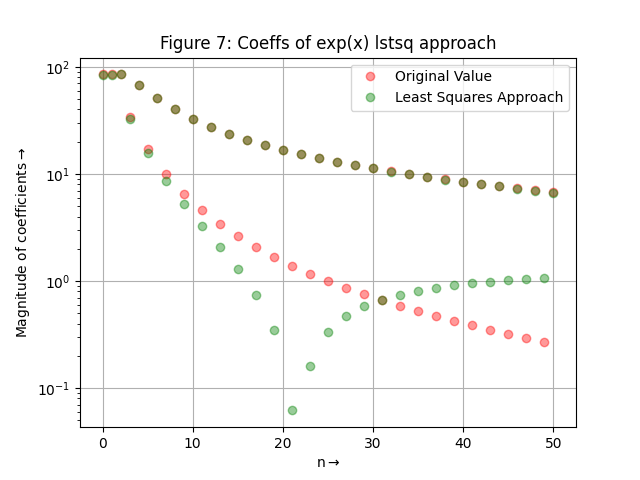
\includegraphics[scale=0.5]{q5-exp-semilog.png} 
    \caption{Q5: \texttt{lstsq} coefficients for $e^x$ (semilog)}
   	\label{fig:lstsq coeff for exp()}
   \end{figure}
   
   \begin{figure}[!tbh]
   	\centering
  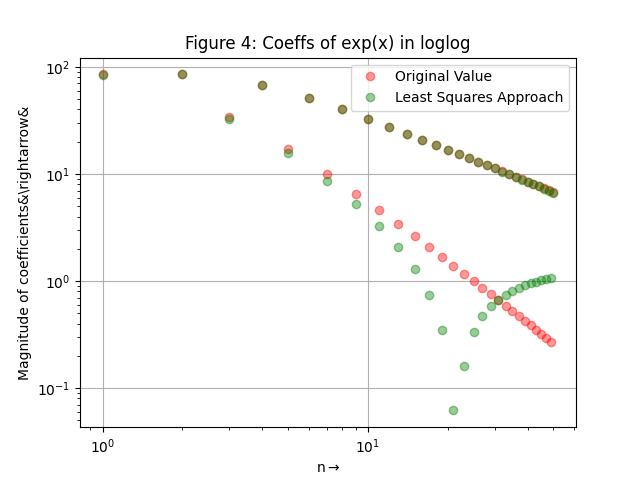
\includegraphics[scale=0.5]{q5-exp-loglog.png} 
    \caption{Q5: \texttt{lstsq} coefficients for $e^x$ (loglog)}
   	\label{fig:lstsq coeff for exp()}
   \end{figure}
 
 Similar procedure for $\cos(\cos(x))$ gives the following plots. 
 
   \begin{figure}[!tbh]
   	\centering
  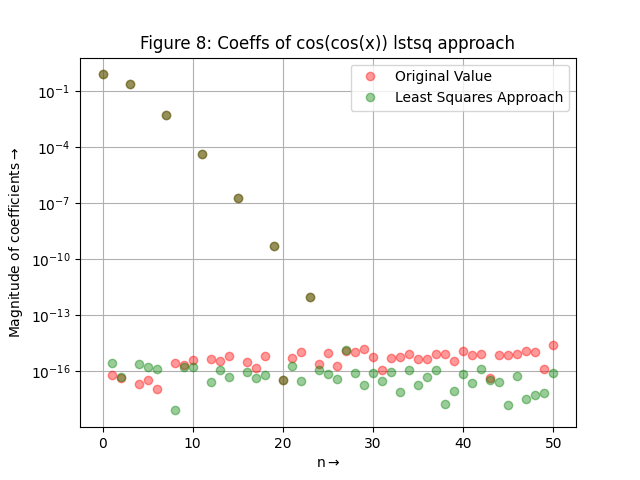
\includegraphics[scale=0.5]{q5-cos-semilog.png} 
    \caption{Q5: \texttt{lstsq} coefficients for $cos(cos(x))$ (semilog)}
   	\label{fig:lstsq coeff for coscos()}
   \end{figure}
   
   \begin{figure}[!tbh]
   	\centering
  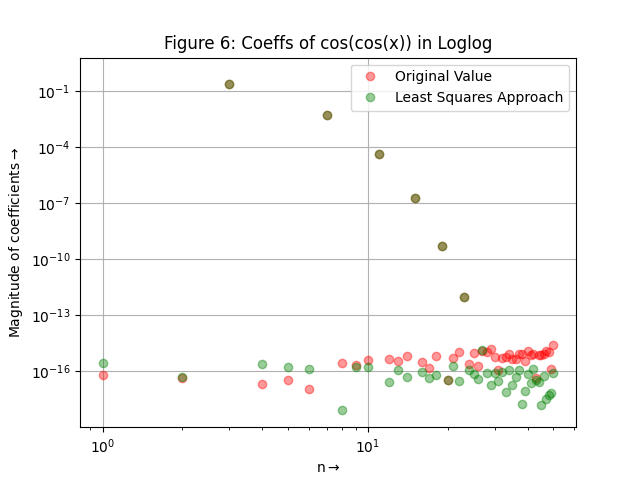
\includegraphics[scale=0.5]{q5-cos-loglog.png} 
    \caption{Q5: \texttt{lstsq} coefficients for $cos(cos(x))$ (loglog)}
   	\label{fig:lstsq coeff for coscos()}
   \end{figure}
   
   \newpage
   \subsection{Question 6: Least Squares Vs Integration!}
   I have calculated the absolute difference between the coefficients obtained from Integration and the least squares approach. The plots and code for both the functions follow.
   
   \begin{verbatim}
   # PART 6: Deviation
# First the exponential
error_exp = coeffs_of_exp - abs(coeff_for_exp_lstsq)
plot(range(51), abs(error_exp), 'ro')
xlabel('n')
ylabel('real coeffs - lstsq coeffs')
title('Deviation in coeffs of exp(x)')
grid()
show()
print(np.amax(abs(error_exp)))

# Second the coscos
error_coscos = coeffs_of_coscos - abs(coeff_for_coscos_lstsq)
plot(range(51), abs(error_coscos), 'ro')
xlabel('n')
ylabel('real coeffs - lstsq coeffs')
grid()
title('Deviation in coeffs of cos(cos(x))')
show()
print(np.amax(abs(error_coscos)))
   \end{verbatim}    
   \begin{figure}[!tbh]
   	\centering
  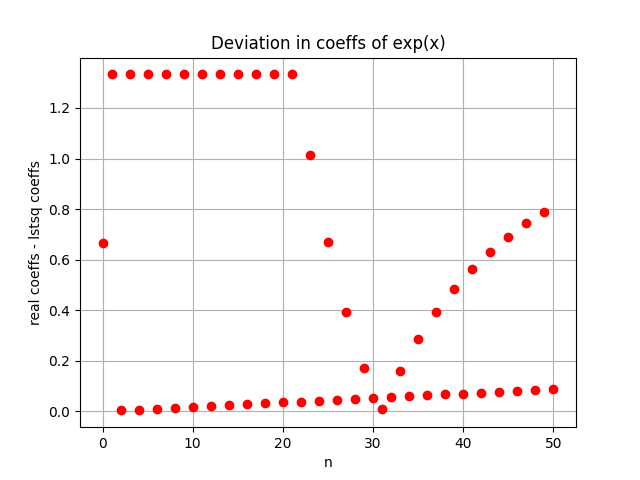
\includegraphics[scale=0.5]{q6-exp.png} 
    \caption{Q6: $e^x$ deviation}
   	\label{fig: deviation exp()}
   \end{figure}
   
   \begin{figure}[!tbh]
   	\centering
  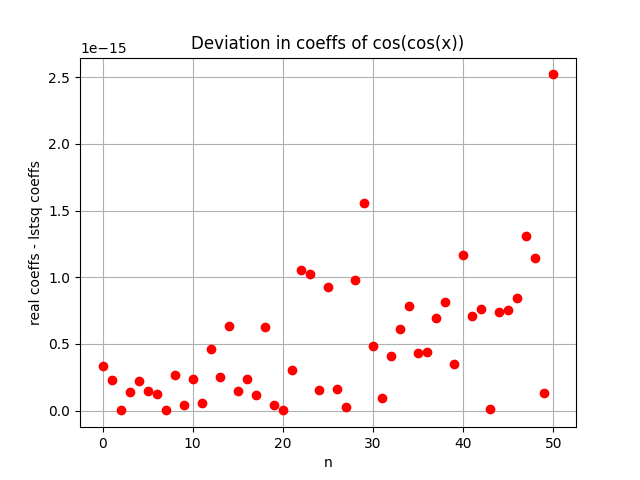
\includegraphics[scale=0.5]{q6-cos.png} 
    \caption{Q6: $cos(cos(x))$ deviation}
   	\label{fig: deviaton coscos()}
   \end{figure}
   
   Maximum deviations are printed by the python program.\\\\
   Max deviation for $e^x$ = 1.3327308703353395\\
   Max deviation for $cos(cos(x))$ = 2.5195381376685242e-15\\
   
   There is appreciable deviation for some of the coefficients of $e^x$ (there is a row of dots above 1.2). 
   The deviation observed for $cos(cos(x))$ coefficients is of the order $10^{-15}$ implying that the least squares and integration coefficients are amazingly close. This difference is because the former is discontinuous at the boundaries but the latter is essentially periodic. 
   
   \subsection{Question 7: Function values' deviation}
   Computing $Ac$ (The function values at $x_{i}$) from the estimated values of $c$. The Python code:
   \begin{verbatim}
   Ac_exp = np.dot(A_mat_for_exp, coeff_for_exp_lstsq)
   Ac_coscos = np.dot(A_mat_for_coscos, 
      coeff_for_coscos_lstsq)
   semilogy(X, Ac_exp, 'go', label='Obtained from lstsq 
      and Fourier', alpha=0.4)
   semilogy(X, exponential(X), label='True Value')
   xlabel('X')
   ylabel('Function values at Xi')
   legend()
   show()

   plot(X, Ac_coscos, 'go', label='Obtained from lstsq 
     and Fourier', alpha=0.4)
   plot(X, coscos(X), label='True Value')
   xlabel('X')
   ylabel('Function values at Xi')
   legend()
   show()
   \end{verbatim}
   
   The function values hence obtained are plotted along with the 'true' values. Significant inaccuracy can be observed for the $e^x$ plot because it would need a larger number of high frequency components to obtain the exact function. On the other hand, the estimated $cos(cos(x))$ function is extremely close to the real values because, in frequency domain, it was almost completely covered up by the first few fourier coefficients (harmonics).
    
   
   \begin{figure}[!tbh]
   	\centering
  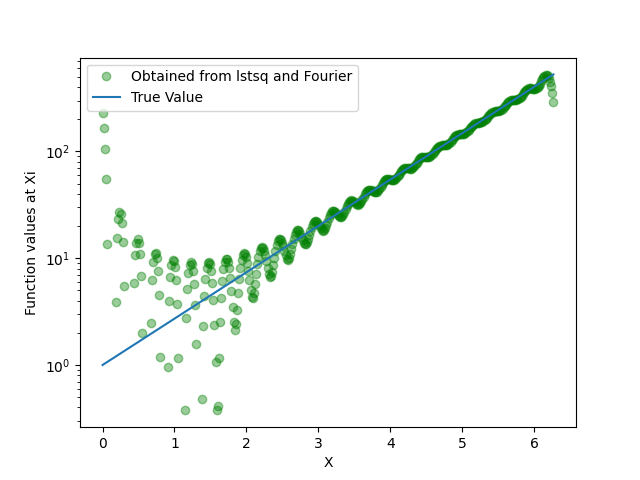
\includegraphics[scale=0.5]{q7-exp.png} 
    \caption{Q7: $e^x$ (semilog)}
   	\label{fig: exp()}
   \end{figure}
   
   
   \begin{figure}[!tbh]
   	\centering
  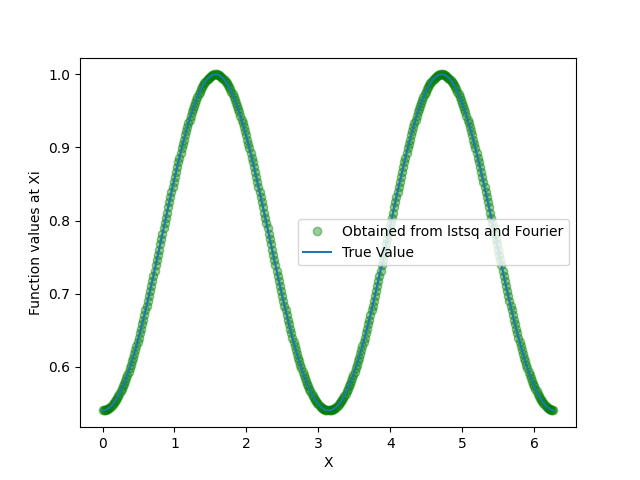
\includegraphics[scale=0.5]{q7-cos.png} 
    \caption{Q7: $cos(cos(x))$}
   	\label{fig: coscos()}
   \end{figure}
   
\newpage
\section{Conclusion}
The aims that I enlisted at the beginning of this report are now seen to have been accomplished. Through every subsection, I analysed how Fourier coefficients will be calculated using scientific Python and every plot gave a deeper insight into their nature. I infer that for a function inherently periodic, the fourier coefficients obtained by both integration and least squares will give accurate results for a finite number of coefficients. However, non-periodic functions when given a periodic extension will create a discontinuity at every integral multiple of Time period. Thus, it will take a greater amount of fourier coefficients to reverse-realise the original function. 


\end{document}



 